\documentclass[a4paper, 11pt]{article}

\usepackage[a4paper,margin=1in]{geometry}
\usepackage[english]{babel}
\usepackage[utf8]{inputenc}
\usepackage[T1]{fontenc}
\usepackage{lmodern}
\usepackage{listings}
\usepackage{graphicx}
\usepackage{amsmath}
\usepackage{framed}
\usepackage{amsfonts}
\usepackage{caption}
\usepackage{subcaption}
\usepackage{listings}
\usepackage{tabularx}
\usepackage{color}
\usepackage[dvipsnames]{xcolor}
\usepackage{fancyhdr}
\usepackage{lastpage}
\usepackage{dirtytalk}
\usepackage{amssymb}
\usepackage{float}
\usepackage[toc,page]{appendix}
\usepackage[backend=biber,style=alphabetic,sorting=ynt]{biblatex}

\addbibresource{references.bib}
\graphicspath{{imgs/}}


\definecolor{morange}{RGB}{237,106,90}
\definecolor{mgreen}{RGB}{63,127,95}
\definecolor{mpurple}{RGB}{127,0,85}

\lstset{
  basicstyle=\small\ttfamily, % Global Code Style
  captionpos=b, % Position of the Caption (t for top, b for bottom)
  extendedchars=true, % Allows 256 instead of 128 ASCII characters
  tabsize=2, % number of spaces indented when discovering a tab
  columns=fixed, % make all characters equal width
  keepspaces=true, % does not ignore spaces to fit width, convert tabs to spaces
  showstringspaces=false, % lets spaces in strings appear as real spaces
  breaklines=true, % wrap lines if they don't fit
  frame=trbl, % draw a frame at the top, right, left and bottom of the listing
  frameround=tttt, % make the frame round at all four corners
  framesep=4pt, % quarter circle size of the round corners
  numbers=left, % show line numbers at the left
  numberstyle=\tiny\ttfamily, % style of the line numbers
  commentstyle=\color{mgreen}, % style of comments
  keywordstyle=\color{mpurple}, % style of keywords
  stringstyle=\color{morange}, % style of strings
}

% TAILLE DES PAGES (A4 serré)

\setlength{\parindent}{0pt}
\setlength{\parskip}{1em}
%% \setlength{\textwidth}{17cm}
%% \setlength{\textheight}{24cm}
%% \setlength{\oddsidemargin}{-.7cm}
%% \setlength{\evensidemargin}{-.7cm}
%% \setlength{\topmargin}{-.5in}


\pagestyle{fancy}
\renewcommand{\headrulewidth}{0pt}
\renewcommand{\footrulewidth}{0.6pt}% default is 0pt
\lhead{}
\rhead{}
\lfoot{Page \thepage\ of \pageref{LastPage}}
\rfoot{Rémi Lespinet, Steeve Vu, Victor Busa}
\cfoot{}
\cfoot{}


\newcounter{cquestion}
\renewcommand{\thecquestion}{\arabic{cquestion}}
\newenvironment{question}
{\par \vspace{0.5em} \noindent \stepcounter{cquestion} \hspace{-1em}
 $\bullet$ \underline{Q\thecquestion :}}
{}

\newenvironment{note}
{\begin{framed} \textbf{Note : }}
{\end{framed}}


% Commandes de mise en page
\newcommand{\file}[1]{\lstinline{#1}}
\newcommand{\name}[1]{\emph{#1}}
\newcommand{\itemi}{\item[$\bullet$]}

\newcommand{\norm}[1]{\|{#1}\|}

% Commandes color
\newcommand{\colgood}[1]{\color{ForestGreen} #1}
\newcommand{\colbad}[1]{\color{BrickRed} #1}


\pagenumbering{arabic}

\title{\textsc{Unsupervised Learning - MVA 2017/2018 \\ \emph{Homework 2}} }
\author{Victor Busa, Steeve Vu, Rémi Lespinet}
\date{}

\begin{document}

\maketitle
\thispagestyle{fancy}

\section{Algorithms implementations}

\subsection{Spectral Clustering}

To compute the affinity, we use the symmetrized $K$-nearest neighbors
gaussian affinity

\begin{equation*}
  w_{ij} = \left\{
    \begin{array}{ll}
      \exp{(-\norm{x_i - x_j})} & \text{ if $x_i$ and $x_j$ are K-neighbors} \\
      0 & \text{ otherwise }
    \end{array}
  \right.
\end{equation*}

Where K-neighbors means that one of $x_i$ is in the $K$ nearest
neighborhood of $x_j$ or vice versa.

We $l_2$ normalize the datas before computing the affinity
matrix, as it is discussed p.158 in \cite{vidal16}. This allows us
to choose $\sigma$ around the unit value.

\subsection{Sparse Subspace Clustering} \label{ss:ssc}

For SSC We choose $\tau = 10 \times \tau_{min}$, where $\tau_{min}$ is defined in \cite{elhamifar09} as:
$$\tau_{min} \triangleq \dfrac{1}{\min\limits_{i} \max\limits_{j \neq i} |y_i^T y_j |}$$

We also had to normalize the matrix returned by the ADMM\_LASSO algorithm using the infinity norm:

$$c_i \leftarrow \dfrac{c_i}{\norm{c_i}_{\infty}}$$

before computing the Affinity matrix: $W = |C| + |C^T|$.

\subsection{K-Subspaces}

For the initialization of the subspace basis $U$, we compute a
Singular Value Decomposition on a random matrix (where each
coefficient is generated with a standard normal distribution).  (We
have tried other methods such as QR decomposition of random matrices
and the dedicated Scikit-learn method \verb+rvs+, but this is slower
since these methods generate full square matrices, and we only need
a small number of orthonormal vectors of high dimension)


For the initialization of mu, we've tried several methods
\begin{itemize}
\item We first initialize mu with $n$ points in the training data
  chosen at random (\verb+init_naive+). We then tried to improve this using the $Kmeans++$
  initialization (taking points iteratively with a probability
  depending on the distances to the set of points already
  chosen) (\verb+init_kmeanspp+).
\item We then tried to sample mu at random using a mutivariate
  gaussian random variable with mean and covariance matching the
  covariance of the data (\verb+init_gaussian+).
\end{itemize}

\section{Face clustering}

\subsection{Tuning the parameters}
\subsubsection{Tuning $\sigma$ and $k$ for Spectral Clustering}

Working on individuals 1-2, we have tuned the parameters $\sigma$ and $k$.

We first fixed $\sigma = 1$ and tune for $k \in [1, 128]$, the results are shown on Figure \ref{fig:sc_tune_k}

\begin{figure}[H]
	\centering
	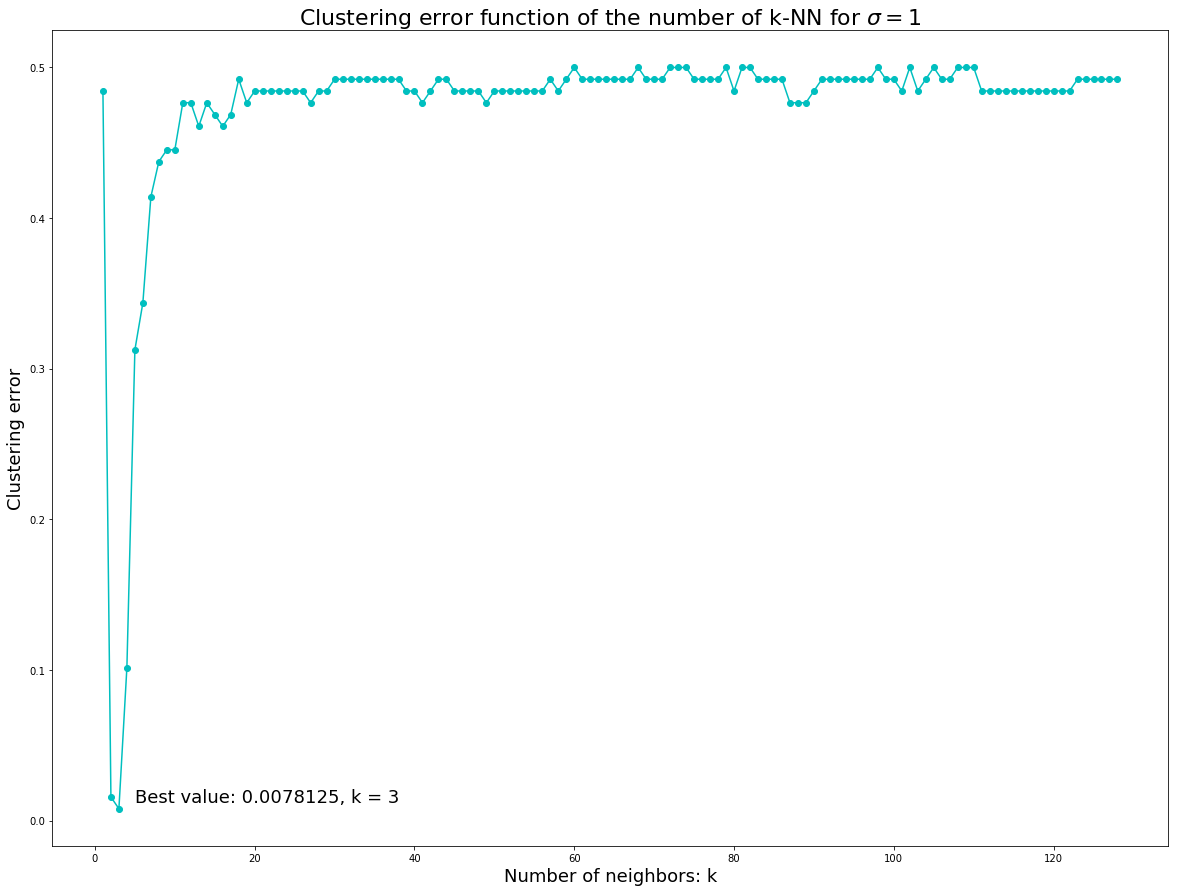
\includegraphics[width=.7\linewidth]{imgs/SC_tune_k.png}
	\caption{Clustering error in function of the number of k nearest-neighbors considered}
	\label{fig:sc_tune_k}
\end{figure}

As shown on Figure \ref{fig:sc_tune_k}, the clustering error is minimal for $k = 3$. Letting $k=3$ we then tune the parameter $\sigma$ for $\sigma$ in the range [0.001, 10]. The Figure \ref{fig:sc_tune_sig} shows the clustering error in function of the parameter $\sigma$.

\begin{figure}[H]
	\centering
	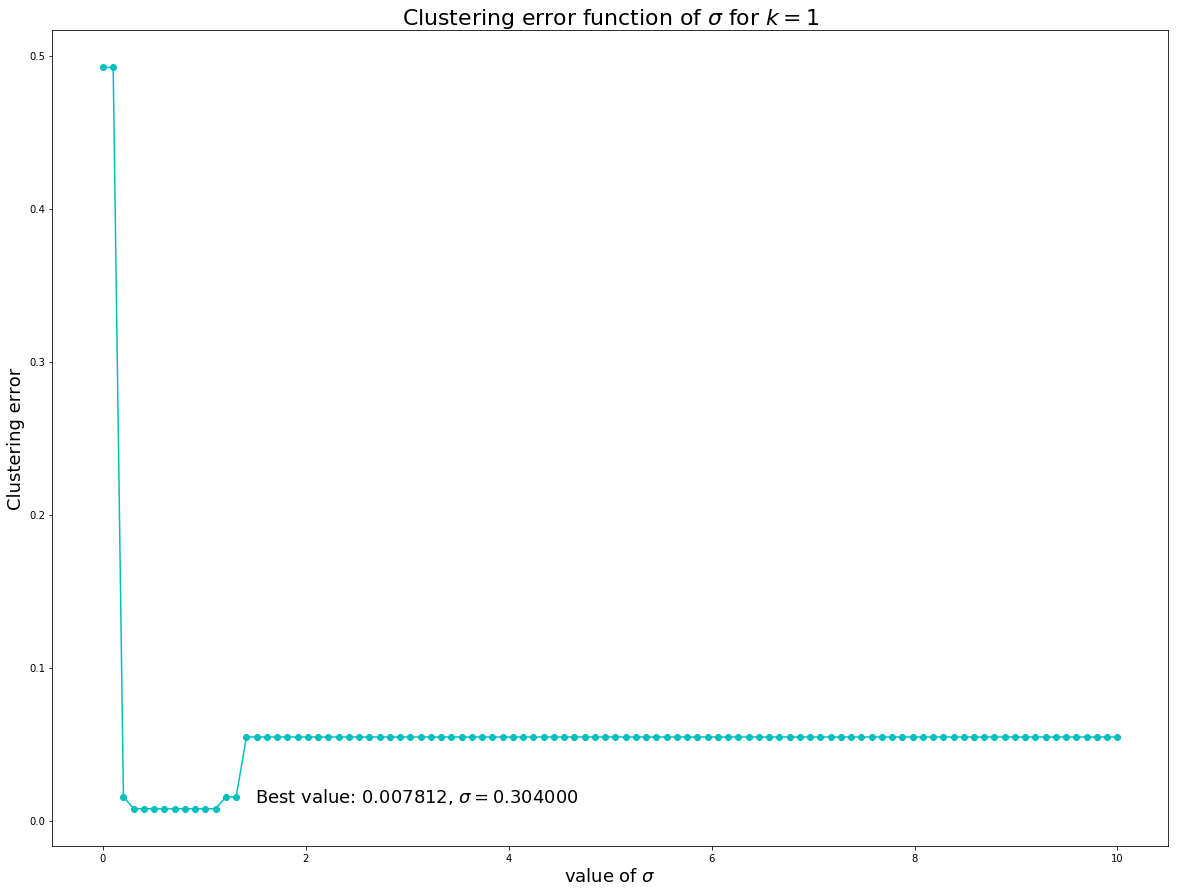
\includegraphics[width=.7\linewidth]{imgs/SC_tune_sigma.png}
	\caption{Clustering error function of $\sigma$ for $k=3$}
	\label{fig:sc_tune_sig}
\end{figure}

\subsubsection{Tuning number of restart and dimensions for $K$-subspaces}

\subsubsection{Varying the dimension of the subspaces}

The figure \ref{fig:k-subspaces-dim} presents the clustering error as a function of the dimension of the subspaces (each subspace dimension argument is the same). The number of restart is fixed to 10.

It appears that choosing 9 for the dimension of each subspace gives best results. This agrees with the proposition that images of a face under different lighting conditions lye in a subspace of dimension 9. Taking a dimension
of 3 also seems to give good results in most cases


\begin{figure}[H]
	\centering
	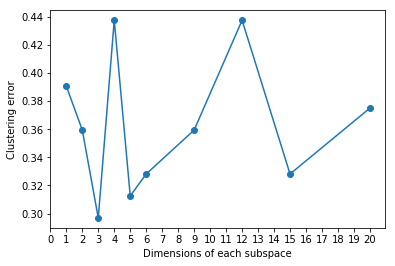
\includegraphics[width=.7\linewidth]{ksubspaces_dim.png}
	\caption{Clustering error for $K$-subspaces as a function of the dimensions on individual 1 and 2 of the dataset (fixed number of restart=10)}
	\label{fig:k-subspaces-dim}
\end{figure}

\textbf{Varying the number of the replicates}

In the figure \ref{fig:k-subspaces-restarts}, we present the results of the clustering error obtained on individual 1 and 2, when we vary the number of replicates (restarts). The dimension for each subspace is fixed to 9.

\begin{figure}[H]
	\centering
	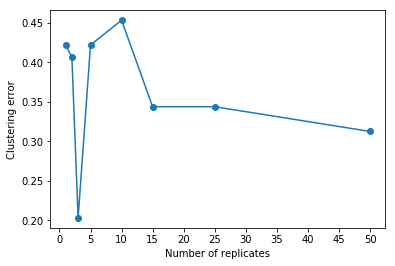
\includegraphics[width=.7\linewidth]{ksubspaces_restarts.png}
	\caption{Clustering error as a function of the number of restarts for $K$-subspaces on individual 1 and 2 of the dataset (fixed number of dimension=9)}
	\label{fig:k-subspaces-restarts}
\end{figure}


\subsubsection{Tuning $\mu_2$ for SSC} \label{sss:tune_ssc}
We fix $\tau$ as $\tau = 10 \times \tau_{min}$ as we emphasized in \ref{ss:ssc}. We then tune the parameter $\mu_2$ for $\mu_2$ varying in
[$1.10^1$, $1.10^6$] in a logarithmic way. The clustering error obtained is displayed on Figure \ref{fig:ssc_tune_mu2}.

\subsection{Clustering error as a function of the number of groups}





\subsubsection{SSC}

\begin{figure}[H]
	\centering
	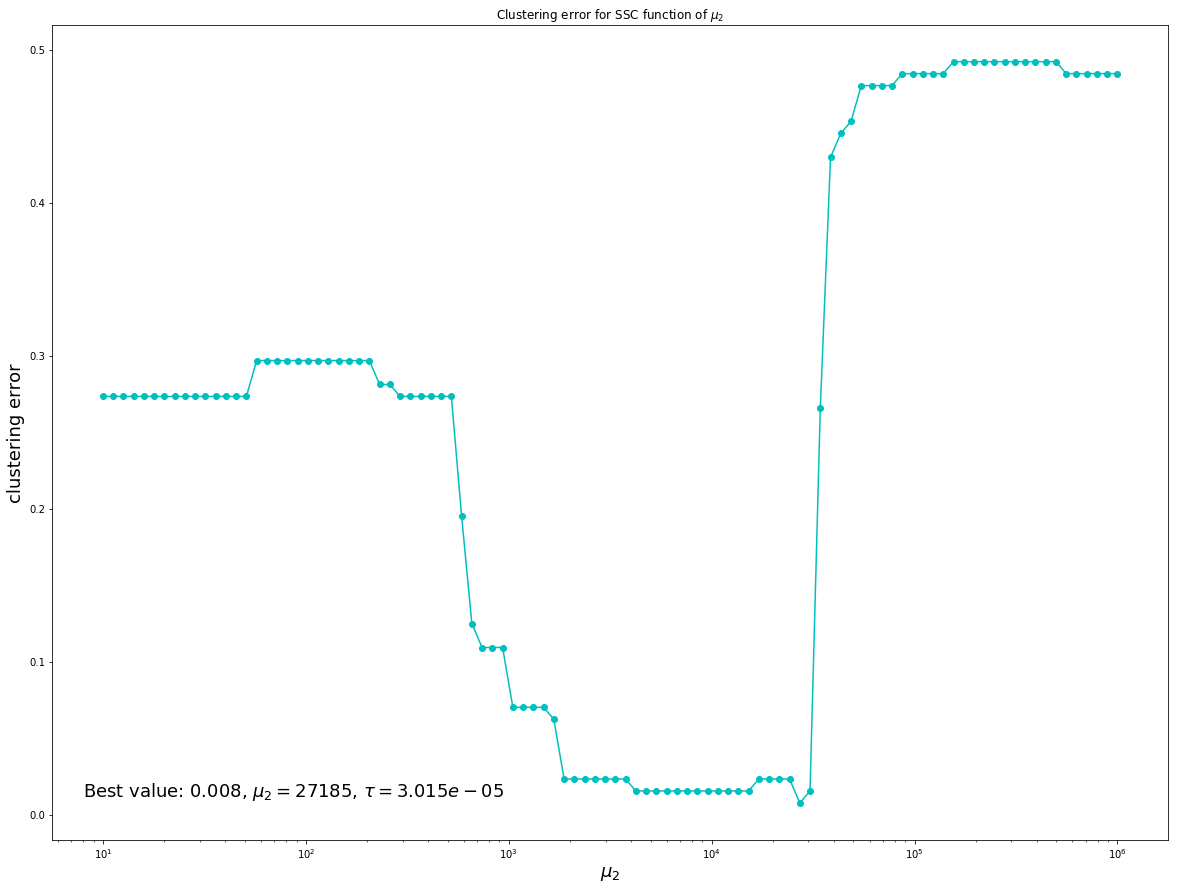
\includegraphics[width=.7\linewidth]{imgs/SSC_tune_mu2.png}
	\caption{Clustering error function of $\mu_2$}
	\label{fig:ssc_tune_mu2}
\end{figure}

\subsection{Results as a function of the number of groups}

\begin{figure}[H]
	\centering
	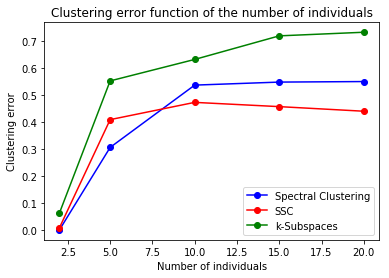
\includegraphics[width=.7\linewidth]{imgs/algos_comparison.png}
	\caption{Clustering error as a function of the number of groups}
	\label{fig:graphs}
\end{figure}



\section{Motion segmentation}

We tuned the hyperparameters for each algorithm in order to get the minimal mean error rate for the 157 videos.

\begin{itemize}
    \item \textbf{Spectral Clustering}: We used $k = 8$ nearest neighbors and $\sigma = 1$
    \item \textbf{$K$-subspaces}: For each subspace $s$ we used $d_s = 3$ with 5 replicates
    \item \textbf{SSC}: Just like the section \ref{sss:tune_ssc}, we chose $\tau = 10\times \tau_{min}$ with a $\mu_2 = 800$. Recall that $\tau_{min}$ depends on the data so it is not fixed.
\end{itemize}

\begin{table}[H]
    \centering
      \caption{Performance for each algorithm on motion segmentation}
    \begin{tabular}{|c|c|c|c|}
        \hline
        Algorithm & Mean & Median & Standard deviation\\
        \hline
        Spectral Clustering & 0.204 & 0.203 & 0.172\\
        \hline
        $K$-subspaces & 0.0991 & 0.0379 & 0.1343\\
        \hline
        SSC & 0.186 & 0.162 & 0.161\\
        \hline
    \end{tabular}
\end{table}


We observe that the results are better on this dataset than on the set of images.
In particular K-subspaces give very good results (on more than $50\%$ of the videos, the clustering error is less than $3\%$)

\section{Organization of the work}

We all wrote all of the algorithms on our side, so that we can easily share and debug our code. We then met to share our results, and write the report. (The 3 python notebook are included in the final archive)

It appears that SSC is not as good as expected on the dataset of images, we may have an error somewhere or we may not have chosen the right parameters.


\newpage
\appendix

\section{Note on the performance of K-Subspaces on the images}

The spectral clustering algorithm is based on the assumption that the
images in the same clusters form (or almost form) a convex component
in the underlying graph. Note that this is wrong in our case, since
the distance between images is the sum of square distances of its
pixels, which is not necessarily smaller for 2 faces of the same
individual than the one for 2 faces of 2 different individuals.  To
illustrate that, the figure \ref{fig:individual-distances} Shows an
image (left) with the top 4 closer faces according to this distance in
the database (and their label). We see that the closest images does
not match the right individual, hence, the graph will most likely be
corrupted.

\begin{figure}[h]
  \centering
  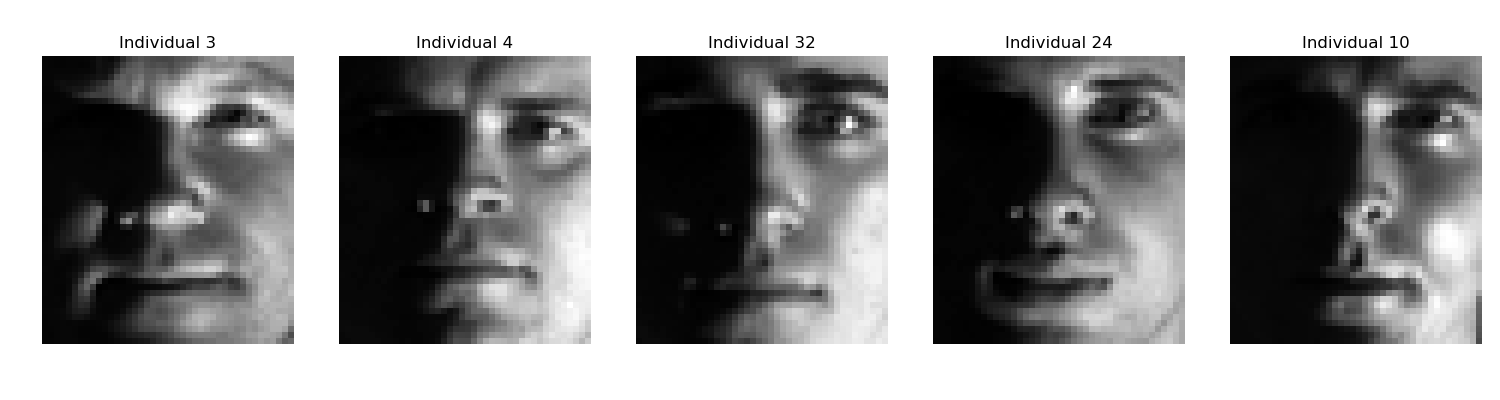
\includegraphics[width=0.8\textwidth]{individual_distances}
  \caption{A data face (left) and its closest 4 faces (sorted from
    left to right) in the database according to the euclidian
    distance}\label{fig:individual-distances}
\end{figure}

We can also illustrate that by computing the affinity on the gradient
of the images instead on the image directly, and we obtain better
results, as shown in the figure \ref{fig:sc-gradient}

\begin{figure}[h]
  \centering
  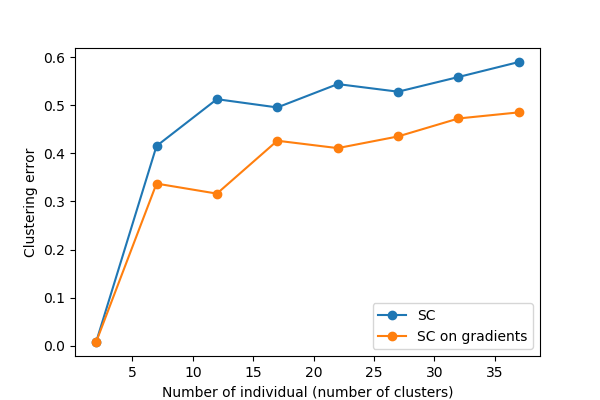
\includegraphics[width=0.7\textwidth]{sc_gradient}
  \caption{Comparison of the performances of the SC classifier applied
    on images, and on their gradients}\label{fig:sc-gradient}
\end{figure}

\newpage
\section{Note on the performance of SSC}
Sparse Spectral Clustering performance doesn't match the performance highlighted p.343 in \cite{vidal16}. This may be due to:
\begin{itemize}
    \item The fact that we implemented SSC for Noisy Data
    \item We don't update the Lagrange multipliers at each iteration of the ADMM\_LASSO algorithm
\end{itemize}

\newpage
\printbibliography

  % \begin{figure}[h]
  %   \centering
  %   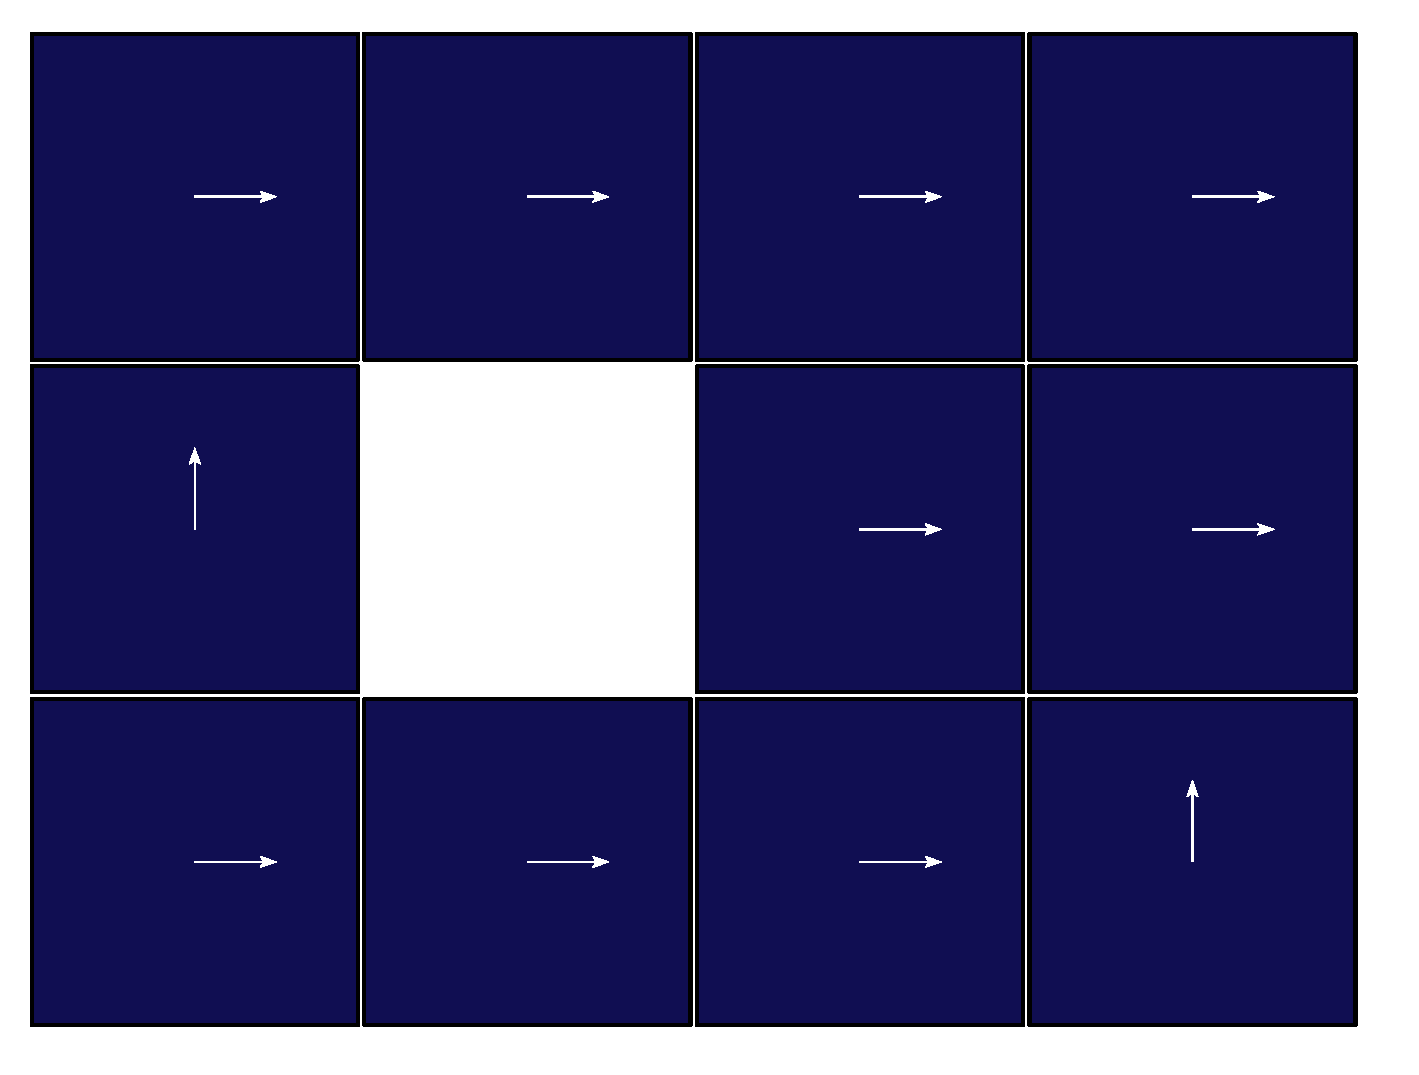
\includegraphics[width=0.7\textwidth]{policy_right_or_up}
  %   \caption{Representation of the policy to evaluate}\label{fig:policy-right-or-up}
  % \end{figure}

\end{document}